\documentclass[paper=a4, fontsize=11pt]{scrartcl} % A4 paper and 11pt font size

%----------------------------------------------------------------------------------------
%	PACKAGES
%----------------------------------------------------------------------------------------
\usepackage[T1]{fontenc} % Use 8-bit encoding that has 256 glyphs
\usepackage{fourier} % Use the Adobe Utopia font for the document - comment this line to return to the LaTeX default
\usepackage[english]{babel} % English language/hyphenation
\usepackage{amsmath,amsfonts,amsthm} % Math packages
\usepackage{sectsty} % Allows customizing section commands
\usepackage{fancyhdr} % Custom headers and footers
\usepackage{xcolor} % Allows 0-255 RGB values
\usepackage{tabularx, outlines, framed, varwidth, enumitem, graphicx, listings, color, qtree, float, subcaption, newfloat}
\usepackage[left=0.5in, right=0.5in, top=3in, bottom=.25in]{geometry}
\geometry{}

%----------------------------------------------------------------------------------------
%	SET CUSTOMIZATIONS AND FUNCTIONS
%----------------------------------------------------------------------------------------
\sectionfont{\centering \normalfont\scshape} % Make all sections centered, the default font and small caps
\pagestyle{fancyplain} % Makes all pages in the document conform to the custom headers and footers
\fancyhead{} % No page header - if you want one, create it in the same way as the footers below
\fancyfoot[L]{} % Empty left footer
\fancyfoot[C]{} % Empty center footer
\fancyfoot[R]{\thepage} % Page numbering for right footer
\renewcommand{\headrulewidth}{0pt} % Remove header underlines
\renewcommand{\footrulewidth}{0pt} % Remove footer underlines
\setlength{\headheight}{0pt} % Customize the height of the header

\DeclareFloatingEnvironment[fileext=lod]{diagram}

\numberwithin{equation}{section} % Number equations within sections (i.e. 1.1, 1.2, 2.1, 2.2 instead of 1, 2, 3, 4)
\numberwithin{figure}{section} % Number figures within sections (i.e. 1.1, 1.2, 2.1, 2.2 instead of 1, 2, 3, 4)
\numberwithin{table}{section} % Number tables within sections (i.e. 1.1, 1.2, 2.1, 2.2 instead of 1, 2, 3, 4)

\graphicspath{{./figures/}}
%\setlength\parindent{0pt} % Removes all indentation from paragraphs - comment this line for an assignment with lots of text

\makeatletter
	\newcommand*\variableheghtrulefill[1][.4\p@]
	{%
		\leavevmode
		\leaders \hrule \@height #1\relax \hfill
		\null
	}
\makeatother

\definecolor{solBase03}{RGB}{000,043,054}
\definecolor{solBase02}{RGB}{007,054,066}
\definecolor{solBase01}{RGB}{088,110,117}
\definecolor{solBase00}{RGB}{101,123,131}
\definecolor{solBase0}{RGB}{131,148,150}
\definecolor{solBase1}{RGB}{147,161,161}
\definecolor{solBase2}{RGB}{238,232,213}
\definecolor{solBase3}{RGB}{253,246,227}
\definecolor{solYellow}{RGB}{181,137,000}
\definecolor{solOrange}{RGB}{203,075,022}
\definecolor{solRed}{RGB}{220,050,047}
\definecolor{solMagenta}{RGB}{211,054,130}
\definecolor{solViolet}{RGB}{108,113,196}
\definecolor{solBlue}{RGB}{038,139,210}
\definecolor{solCyan}{RGB}{042,161,152}
\definecolor{solGreen}{RGB}{133,153,000}

\lstdefinestyle{mystyle}{
	% To Match
	sensitive=true,	
	%
	% Add border
	frame=lines,
	%
	% Add Margin
	xleftmargin=\parindent,
	%
	% Put extra space under caption
 belowcaptionskip=1\baselineskip,
 %
 % Colors:
	backgroundcolor=\color{solBase3},
 basicstyle=\color{solBase00}\footnotesize,
 keywordstyle=\color{solCyan},
 commentstyle=\color{solBase1},
 stringstyle=\color{solBlue},
 numberstyle=\color{solViolet},
 identifierstyle=\color{solBase00},
 %
 % Formatting Options
 breakatwhitespace=false,
 breaklines=true, % break long lines
 captionpos=b,
 keepspaces=true,
 numbers=left,
 numbersep=5pt,
 showspaces=false,
 showstringspaces=false,
 showtabs=false,
 tabsize=4
}

\lstdefinestyle{smallstyle}{
	% To Match
	sensitive=true,	
	%
	% Add border
	frame=lines,
	%
	% Add Margin
	xleftmargin=\parindent,
	%
	% Put extra space under caption
 belowcaptionskip=1\baselineskip,
 %
 % Colors:
	backgroundcolor=\color{solBase3},
 basicstyle=\color{solBase00}\scriptsize,
 keywordstyle=\color{solCyan},
 commentstyle=\color{solBase1},
 stringstyle=\color{solBlue},
 numberstyle=\color{solViolet},
 identifierstyle=\color{solBase00},
 %
 % Formatting Options
 breakatwhitespace=false,
 breaklines=false, % break long lines
 captionpos=b,
 keepspaces=true,
 numbers=left,
 numbersep=5pt,
 showspaces=false,
 showstringspaces=false,
 showtabs=false,
 tabsize=2
}
 
\lstset{style=mystyle}

%----------------------------------------------------------------------------------------
%	USEFUL COMMANDS
%----------------------------------------------------------------------------------------
%	\makebox[\textwidth][c]{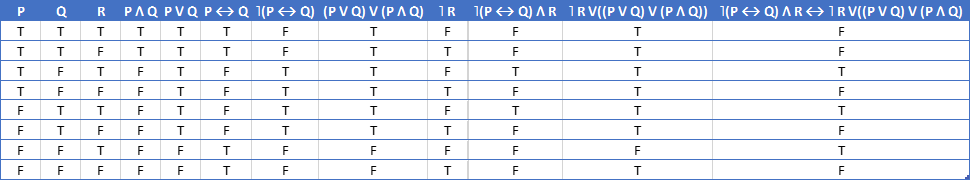
\includegraphics[width=.9\paperwidth]{p2-table}}

%	\newgeometry{top=.75in, bottom=.75in, left=.25in,right=.25in}
%	\newgeometry{top=.75in, bottom=.75in, left=1.25in,right=1.25in}

%	\lstinputlisting[firstline=0, language=C, style=mystyle]{CMPSC360_Homework.cpp}

%\Tree
%	[.<root> [.<left> ][.<middle> ][.<right> ]]

%----------------------------------------------------------------------------------------
%	TITLE SECTION
%----------------------------------------------------------------------------------------

\newcommand{\horrule}[1]{\rule{\linewidth}{#1}} % Create horizontal rule command with 1 argument of height
% \title{Template: Homework 1}
\title{	
\normalfont \normalsize 
%\textsc{Rutgers University, Real Analysis I} \\ [25pt] % Your university, school and/or department name(s)
\horrule{0.5pt} \\[0.4cm] % Thin top horizontal rule
\huge STAT 461: Homework 5 \\ % The assignment title
\horrule{2pt} \\[0.5cm] % Thick bottom horizontal rule
}

\author{\textbf{\underline{Name:}}Kyle Salitrik | \textit{\textbf{\underline{ID\#:}} 997543474} | \textit{\textbf{\underline{PSU ID:}} kps168}} % Your name

\date{\normalsize\today} % Today's date or a custom date

\begin{document}

\maketitle % Print the title

%----------------------------------------------------------------------------------------
%	PROBLEM 1
%----------------------------------------------------------------------------------------
\newgeometry{top=.75in, bottom=.75in, left=1.25in,right=1.25in}
\section*{\variableheghtrulefill[.25ex]\quad Problem 1 \quad\variableheghtrulefill[.25ex]}
\subsection*{a)}
\begin{flalign*}
Y_{it} &= \mu + \tau_i + \epsilon_{it},\quad \epsilon_{it} \sim N(0,\sigma^2) & \\
i &= A,B,C & \\
t &= 1, \dots ,r_i; \quad r_A = r_B = r_C = 2 &
\end{flalign*}

\subsection*{b)}
\begin{flalign*}
\overline{Y}_{B\cdot} &= \frac{5-1}{2} = 4&\\
\overline{Y}_{B\cdot} &\sim N\left(4,\frac{\sigma^2}{2}\right) &
\end{flalign*}

\subsection*{c)}
\begin{flalign*}
\overline{Y}_{A\cdot} &= \frac{-14-4}{2} = -9&\\
\overline{Y}_{B\cdot} &= \frac{5-1}{2} = 2&\\
\overline{Y}_{C\cdot} &= \frac{-2+6}{2} = 2&\\
\overline{Y}_{\cdot\cdot} &= \frac{-14-4+5-1-2+6}{6} = \frac{-5}{3}&\\
\text{SSE} &= \sum_{i=1}^{v}\sum_{t=1}^{r_i} \left(\overline{Y}_{it} - \overline{Y}_{i\cdot}\right)^2 &\\
&= \left(-14+9\right)^2 + \left(-4+9\right)^2 + \left(5-2\right)^2 + \left(-1-2\right)^2 + \left(-2-2\right)^2 + \left(6-2\right)^2 &\\
&= 100 &\\
\text{SST} &= \sum_{i=1}^{v} r_i \left(\overline{Y}_{i\cdot} - \overline{Y}_{\cdot\cdot}\right)^2 &\\
&= 2\left(-9 - \frac{-5}{3}\right)^2 + 2\left(2 - \frac{-5}{3}\right)^2 + 2\left(2 - \frac{-5}{3}\right)^2 & \\
&= \frac{484}{3} \approx 161.\overline{333} &\\
\text{SSTOT} &= \sum_{i=1}^{v}\sum_{t=1}^{r_i} \left(\overline{Y}_{it} - \overline{Y}_{i\cdot}\right)^2 &\\
&= \left(-14-\frac{-5}{3}\right)^2 + \left(-4-\frac{-5}{3}\right)^2 + \left(5-\frac{-5}{3}\right)^2 + \left(-1-\frac{-5}{3}\right)^2 + \left(-2-\frac{-5}{3}\right)^2 + \left(6-\frac{-5}{3}\right)^2 &\\
&= \frac{784}{3} \approx 261.\overline{333} &
\end{flalign*}

\subsection*{d)}
\begin{flalign*}
\widehat{\sigma^2} & \approx \frac{\text{SSE}}{n-v} = \frac{756}{6-3} = 252 &
\end{flalign*}

\subsection*{e)}
\begin{flalign*}
\widehat{\Delta}_{AC} &= \overline{Y}_{A\cdot} - \overline{Y}_{C\cdot} = -9 - 2 = -11 &
\end{flalign*}

\subsection*{f)}
\begin{flalign*}
\overline{Y}_{A\cdot} - \overline{Y}_{C\cdot} & \sim N(\mu + \tau_A, \sigma^2) + N(-\mu - \tau_C, \sigma	^2) = N(0, 2\sigma^2) &
\end{flalign*}

\subsection*{g)}
\begin{flalign*}
\frac{\overline{Y}_{A\cdot} - \overline{Y}_{C\cdot}}{K(\sigma)} & \sim N(0, 2\left(\frac{1}{K(\sigma)}\right)^2 \sigma^2) & \\
K(\sigma) & = \sqrt{2}\sigma &
\end{flalign*}

\subsection*{h)}
\begin{flalign*}
\frac{\text{SSE}}{\sigma^2} & \sim \chi^2_{n-v} &
\end{flalign*}

\subsection*{i)}
\begin{flalign*}
\frac{\left(\overline{Y}_{A\cdot}-\overline{Y}_{C\cdot}\right)^2/\left(K(\sigma)\right)^2}{\text{SSE}/\left[\left(n-v\right)\sigma^2\right]} & \sim F_{1,(n-v)} &
\end{flalign*}

\subsection*{j)}
Under the null hypothesis of $H_0: \tau_A = \tau_B = \tau_C$, we use the test statistic $T^* = \frac{\text{SST}/(v-1)}{\text{SSE}/(n-v)}$ where $T^* \sim F_{(v-1),(n-v)}$.

In general:

\begin{tabularx}{\textwidth}{| X | X | X | X | X |}
\hline
& DF & Sum Sq & Mean Sq & F-Value \\ \hline
Treatment & v-1 & SST & $\text{SST}/(v-1)$ & $\frac{\text{SST}/(v-1)}{\text{SSE}/(n-v)}$ \\ \hline
Error & n-v & SSE & $\text{SSE}/(n-v)$ & NA\\ \hline
Total & n-1 & SSTOT & NA & NA \\ \hline
\end{tabularx}
\newline
\newline
For our case:

\begin{tabularx}{\textwidth}{| X | X | X | X | X |}
\hline
& DF & Sum Sq & Mean Sq & F-Value \\ \hline
Treatment & $2$ & $\frac{484}{3}$ & $\frac{242}{3}$ & $\frac{121}{50}$ \\ \hline
Error & $3$ & $100$ & $\frac{100}{3}$ & \\ \hline
Total & $5$ & $\frac{784}{3}$ & NA & NA \\ \hline
\end{tabularx}

\subsection*{k)}
Based on the below output from R, we can conclude that there is no significant difference in the response of the three populations. In this case, $H_0$ should not be rejected.

\lstinputlisting[language=]{listings/hw5_q1_k.txt}

\subsection*{l)}
Examining the pairwise comparisons for the variables, we can see that none of the p-values are significant for any of the contrasts. This confirms that there is no significant difference between the treatments of the 3 populations.

\begin{flalign*}
H_0:& \tau_A = \tau_B \quad H_A: \tau_A \neq \tau_B &\\
H_0:& \tau_A = \tau_C \quad H_A: \tau_A \neq \tau_C &\\
H_0:& \tau_B = \tau_C \quad H_A: \tau_B \neq \tau_C &\\
T^* &= \frac{\sqrt{\frac{r_i+r_j}{r_i r_j}}\left(\overline{Y}_i - \overline{Y}_j\right)}{\sqrt{SSE/\left(n-v\right)}}&\\
T^* &\sim t_{n-v} = t_3 &
\end{flalign*}
\lstinputlisting[language=]{listings/hw5_q1_l.txt}


%----------------------------------------------------------------------------------------
%	PROBLEM 2
%----------------------------------------------------------------------------------------
\section*{\variableheghtrulefill[.25ex]\quad Problem 2 \quad\variableheghtrulefill[.25ex]}
\begin{flalign*}
H_0:& \tau_{reg} = \tau_{deo} \quad H_A: \tau_{reg} \neq \tau_{deo} &\\
H_0:& \tau_{reg} = \tau_{moi} \quad H_A: \tau_{reg} \neq \tau_{moi} &\\
H_0:& \tau_{deo} = \tau_{moi} \quad H_A: \tau_{deo} \neq \tau_{moi} &\\
T^* &= \frac{\sqrt{\frac{r_i+r_j}{r_i r_j}}\left(\overline{Y}_i - \overline{Y}_j\right)}{\sqrt{SSE/\left(n-v\right)}}&\\
T^* &\sim t_{n-v} = t_9 &
\end{flalign*}

Examining the ANOVA table, one can see that there is a significant difference between at least one pair of treatment. Therefore, we reject $H_0$ and must examine further to determine which treatments are significant.

Looking at the pairwise comparisons, we can observe that the deodorant soap lost less than the regular soap, and that the moisturizing soap also lost less than the regular soap. However, there was no significant difference between the moisturizing and deodorant soaps.

\lstinputlisting[language=]{listings/hw5_q2.txt}

%----------------------------------------------------------------------------------------
%	PROBLEM 3
%----------------------------------------------------------------------------------------
\section*{\variableheghtrulefill[.25ex]\quad Problem 3 \quad\variableheghtrulefill[.25ex]}
\begin{flalign*}
H_0:& \tau_{0} = \tau_{1} \quad H_A: \tau_{0} \neq \tau_{1} &\\
H_0:& \tau_{0} = \tau_{2} \quad H_A: \tau_{0} \neq \tau_{2} &\\
H_0:& \tau_{0} = \tau_{3} \quad H_A: \tau_{0} \neq \tau_{3} &\\
H_0:& \tau_{1} = \tau_{2} \quad H_A: \tau_{1} \neq \tau_{2} &\\
H_0:& \tau_{1} = \tau_{3} \quad H_A: \tau_{1} \neq \tau_{3} &\\
H_0:& \tau_{2} = \tau_{3} \quad H_A: \tau_{2} \neq \tau_{3} &\\
T^* &= \frac{\sqrt{\frac{r_i+r_j}{r_i r_j}}\left(\overline{Y}_i - \overline{Y}_j\right)}{\sqrt{SSE/\left(n-v\right)}}&\\
T^* &\sim t_{n-v} = t_{28} &
\end{flalign*}

The p-value obtained from the ANOVA is extremely large, indicating that $H_0$ should not be rejected. Continuing to look at the pairwise comparisons, the p-values for each contrast are also very large, indicating that there is no difference between the treatments.

\lstinputlisting[language=]{listings/hw5_q3.txt}

\newpage
\section*{Code Appendix}
\lstinputlisting[language=R]{461_hw5.R}

\end{document}